\documentclass[10pt,twoside,a4paper,fleqn]{report}
\usepackage[english,st]{rpg} % select type {semester}/bachelor/master thesis: {st}/bt/mt

% Page header (don't change)____________________________________________________
\setlength{\parindent}{0em}                 % Disable parindent
\rhead[\nouppercase{\rightmark}]{\thepage}  % Special headings
\lhead[\thepage]{\nouppercase{\leftmark}}   % Special headings
\cfoot{}                                    % Special headings

%%%%%%%% Hint %%%%%%%%%%%
% Define your custom stuff here, e.g. Symbols that you are using. If you define them here it is easy to change them later on if you run into a nomenclature conflict.
\newcommand{\mysymbol}[0]{\mathbf{S}_{my}}   % custom symbol which can easily be changed if necessary
\newcommand{\bomega}[0]{\boldsymbol{\omega}} % bold greek letter
\newcommand{\bSymb}[1]{\mathbf{#1}}			% toy example with one argument



% Title page (please fill in)___________________________________________________
\title{RPG Thesis Template}

\studentA{Hans Muster}
\ethidA{97-906-739}
\emailA{muster@student.ethz.ch}

% \studentB{Second Student}
% \ethidB{12-345-678}
% \semesterB{9}
% \emailB{second@student.ethz.ch}

\supervision{First Supervisor\\ Second Supervisor}
\date{January 2013}

\infopage
\declaration

% Begin document________________________________________________________________
\begin{document}
\maketitle 							      % Create title page

% Preamble______________________________________________________________________
\pagenumbering{roman} 				% Begin roman page numbering (i,ii,...)
%---------------------------------------------------------------------------
% Table of contents

 \setcounter{tocdepth}{2}
 \tableofcontents
 \cleardoublepage

%---------------------------------------------------------------------------
% List of Figures

 % \addcontentsline{toc}{chapter}{List of Figures}
 % \listoffigures
 % \clearpage

%---------------------------------------------------------------------------
% List of Tables

 % \addcontentsline{toc}{chapter}{List of Algorithms}
 % \listofalgorithms
 % \clearpage

%---------------------------------------------------------------------------
% Abstract

\chapter*{Abstract}
 \addcontentsline{toc}{chapter}{Abstract}

  Compress the introduction in a few key sentences. No more than half a page.

 \cleardoublepage

%---------------------------------------------------------------------------
% Symbols

% \chapter*{Nomenclature}\label{chap:symbole}
% \addcontentsline{toc}{chapter}{Nomenclature}

% \section*{Notation}
%   \begin{tabbing}
%     \hspace*{1.6cm}   \= \kill
%     $a$                \> a scalar \\[0.5ex]
%     $\mathbf{a}$       \> a vector \\[0.5ex]
%     $\mathbf{A}$       \> a matrix \\[0.5ex]
%     $||.||$            \> the $L_2$-norm \\[0.5ex]
%     $\mathbf{J}$       \> the Jacobian \\[0.5ex]
%     $\mathbf{H}$       \> the Hessian \\[0.5ex]
%     $\mathbf{R}_{BI}$  \> rotation from $I$ to $B$ \\[0.5ex]
%     $\mathbf{T}_{BI}$  \> coordinate transformation from $I$ to $B$ \\[0.5ex]
%     $_I\mathbf{t}_{IB}$\> translation from $I$ to $B$, expressed in coordinate system $I$ \\[0.5ex]
%   \end{tabbing}

% \section*{Acronyms and Abbreviations}
%   \begin{tabbing}
%     \hspace*{1.6cm}  \= \kill
%     BA      \> Bundle Adjustment \\[0.5ex]
%     DoF     \> Degree of Freedom \\[0.5ex]
%     IMU     \> Inertial Measurement Unit \\[0.5ex]
%     LM      \> Levenberg-Marquardt \\[0.5ex]
%     LS      \> Least Squares \\[0.5ex]
%     LUT     \> Look-up-table \\[0.5ex]
%     MAV     \> Micro Aerial Vehicle \\[0.5ex]
%     RANSAC  \> Random Sampling Consensus \\[0.5ex]
%     ROS     \> Robot Operating System, www.ros.org \\[0.5ex]
%     RPG     \> Robotics and Perception Group \\[0.5ex]
%     SLAM    \> Simultaneous Localization and Mapping \\[0.5ex]
%     VO      \> Visual Odometry \\[0.5ex]
%   \end{tabbing}

% \clearpage

%---------------------------------------------------------------------------


% Chapters______________________________________________________________________
\pagestyle{fancy}             % Fancy headings
\pagenumbering{arabic}				% Begin arabic page numbering (1,2,...)

\chapter{Introduction}\label{sec:introduction}

Describe the problem and the motivation for this research.

\section{Related Work}\label{sec:related_work}

Describe the current state of the art. Provide all neccessary citations.
\chapter{Approach}\label{sec:approach}

Describe the main steps in your algorithm. An illustration is always helpful.\\

Here are some \LaTeX~tips:


\section{Headings}

  Your report can be structured using several different types of headings. Use the commands \textbackslash\texttt{chapter}\{.\}, \textbackslash\texttt{section}\{.\}, \textbackslash\texttt{subsection}\{.\}, and \textbackslash\texttt{subsubsection}\{.\}. Use the asterisk symbol \texttt{*} to suppress numbering of a certain heading if necessary, for example, \textbackslash\texttt{section*}\{.\}.


\section{References}\label{sec:references}

  References to literature are included using the command \textbackslash\texttt{cite}\{.\}. For example \cite{KleinMurray2007,Strasdat2010WhyFilter}. Your references must be entered in the file \texttt{bibliography.bib}. Making changes or adding new references in the bibliography file can be done manually or by using specialized software such as \textit{JabRef} which is free of charge.

  Cross-referencing within the text is easily done using \textbackslash\texttt{label}\{.\} and \textbackslash\texttt{ref}\{.\}. For example, this paragraph is part of chapter~\ref{sec:approach}; more specifically on page~\pageref{sec:references}.

\section{Writing Equations}\label{sec:math}

  The most common way to include equations is using the \texttt{equation} environment. Use \textbackslash\texttt{eqref}\{.\} to reference an equation, e.g. \eqref{eq:leastsquares}.
  \begin{equation}\label{eq:leastsquares}
      \begin{aligned}
        C(\mathbf{x}) &= \frac{1}{2} \ \sum_{i \in \mathcal I} \sum_{k \in \mathcal K_i} \mathbf{e}_{i,k}(\mathbf{x})^T \ \mathbf{W}_{i,k}  \ \mathbf{e}_{i,k}(\mathbf{x})  \\
        \hat{\mathbf{x}}^{LS} &= \text{argmin}_\mathbf{x} \ C(\mathbf{x}),
      \end{aligned}
  \end{equation}

  \begin{equation}\label{eq:se3}
    \mathtt{T}_i = \begin{bmatrix}\mathbf{R}_i & \mathbf{p}_i \\ 0 & 1\end{bmatrix} \qquad \text{with} \quad \mathbf{R}_i \in SO(3), \ \ \mathbf{p} \in \mathbb{R}^3.
  \end{equation}

\section{Including Graphics}\label{sec:epsgraph}
  The easiest way to include figures in your document is to use pdf figures if you use \texttt{pdflatex} to compile. Figure \ref{img:notation} was created with the use of the open source program \texttt{ipe}.

  \begin{figure}[h]
     \centering
     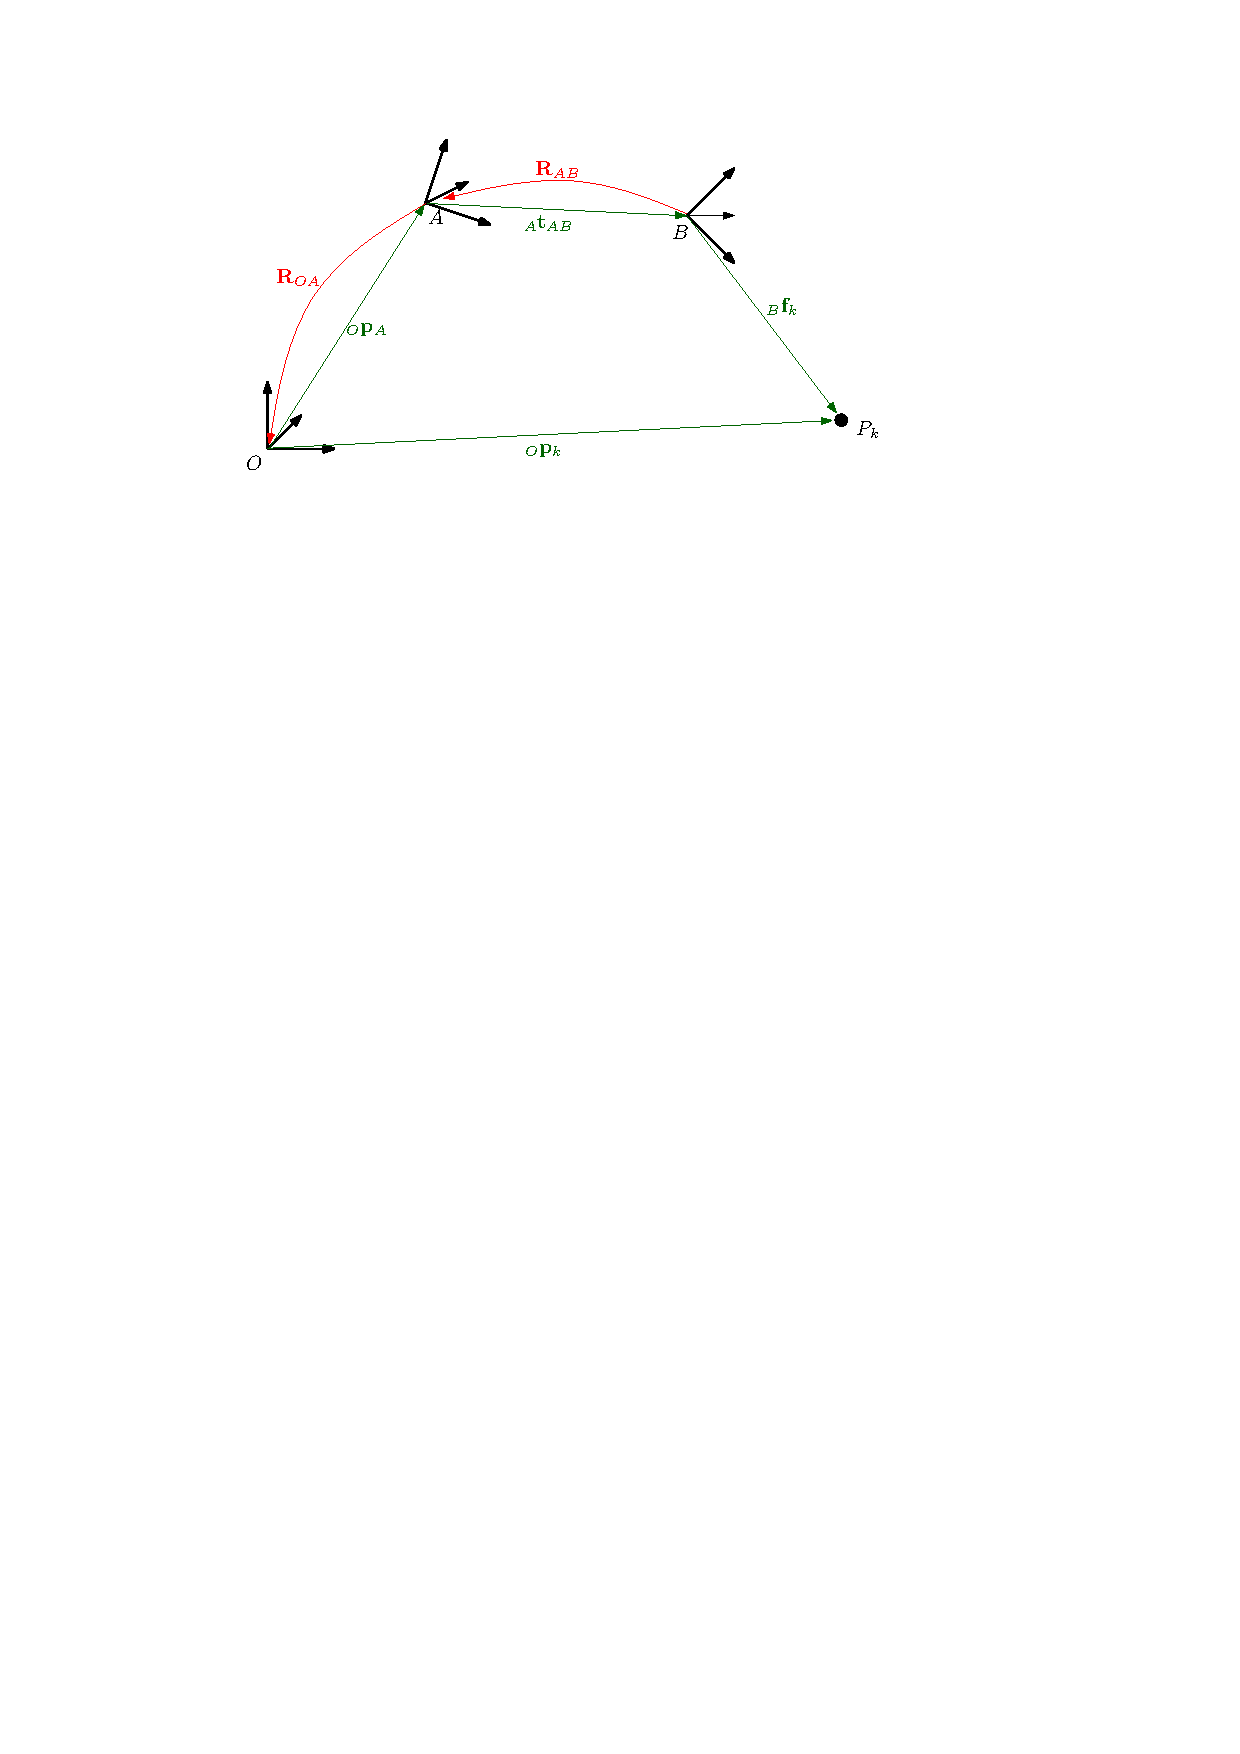
\includegraphics[width=0.6\textwidth]{img/notation.pdf}
     \caption{Example of a figure.}
     \label{img:notation}
  \end{figure}


\section{Including Code in your Document}

  You may include samples from your Matlab code using the \texttt{lstlistings} environment, for example
  \lstset{language=Matlab,numbers=none}
  \begin{lstlisting}[frame=lines, caption=Matlab Example, label=matlabexample]
  % Evaluate y = 2x
  for i = 1:length(x)

    y(i) = 2*x(i);

  end
  \end{lstlisting}

  \lstset{language=C++,numbers=none,caption=C++ Example, label=cppexample}
  \begin{lstlisting}[frame=lines]
  % sum all elements in a list
  int sum=0;
  for(list<int>::iterator it=mylist.begin(); it!=mylist.end(); ++it)
    sum += *it;
  \end{lstlisting}
\chapter{Experiments}\label{sec:experiments}

Provide numerical results, plots and timings. Interpret the data.

\begin{figure}[h]
   \centering
   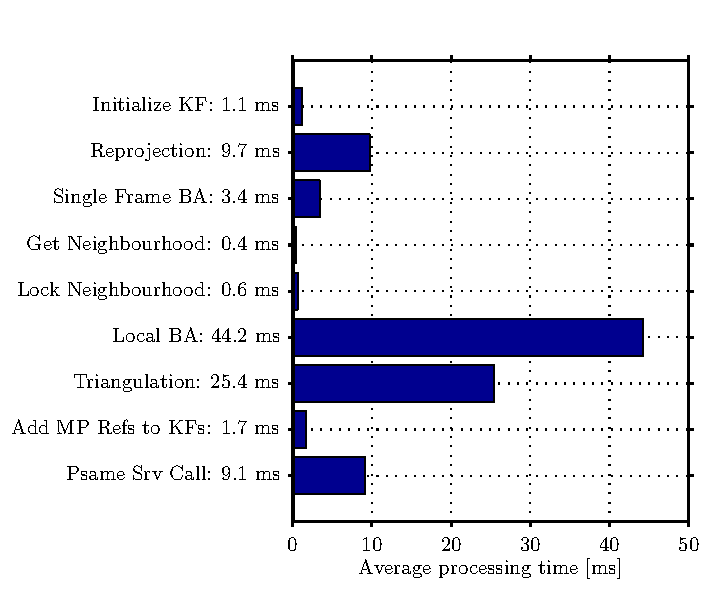
\includegraphics[width=0.75\textwidth]{img/processing_time.pdf}
   \caption{Example of a figure.}
   \label{img:timing}
\end{figure}
\chapter{Discussion}\label{sec:discussion}

Explain both, the advantages and limitations of your approach.

\section{Future Work}\label{sec:future_work}

How would you extend the work? Can you propose another approach?

\cleardoublepage

% Appendix______________________________________________________________________
\appendix

\chapter{Something}\label{sec:something}

In the appendix you can provide some more data, a tutorial on how to run your code, a detailed proof etc.

\cleardoublepage

% Bibliography__________________________________________________________________

\bibliographystyle{plain}
\bibliography{bibtex/references.bib}

\end{document}
